\section{问题四的模型建立与求解}

\subsection{电价数据的周期结构分析}

设 $\lambda_{d,t}$ 为第 $d$ 天第 $t$ 个 10 分钟时段的实际电价（元/kWh），$d=1,\dots,365$，$t=1,\dots,144$。按星期分类求平均，可得各类星期的典型电价曲线，如图~\ref{fig:q4_periodic} 左图所示。日内分时电价呈稳定的阶梯结构，工作日与周末的价格水平存在明显差异。

将全年电价按时间顺序展开为 10 分钟序列 $x_n$（$n=1,\dots,N$，$N=365\times144$），样本自相关函数为

\begin{equation}
  \widehat\rho(k) = \frac{\displaystyle\sum_{n=k+1}^{N}(x_n-\bar x)(x_{n-k}-\bar x)}{\displaystyle\sum_{n=1}^{N}(x_n-\bar x)^2},
  \label{eq:q4_acf}
\end{equation}

式中：$x_n$ 为第 $n$ 个 10 分钟时段的电价（元/kWh）；$\bar x$ 为序列均值；$k$ 为滞后阶数。一天包含 144 个 10 分钟时段，因此第 $h$ 个整日滞后的自相关系数即 $\widehat\rho(144h)$。计算结果如图~\ref{fig:q4_periodic} 右图所示：第 1、7 个整日滞后分别为 0.9299 与 0.9576，第 14、21、28 个整日滞后分别为 0.9260、0.8947 与 0.8634，均明显高于其相邻的非整周滞后，形成整周局部峰值。据此，把过去 4 个同星期、同时刻的价格作为 0:00 全天预测的输入变量。

\begin{figure}[H]
  \centering
  
\includegraphics[width=0.485\textwidth]{../figures/问题四/问题四_典型星期电价曲线.pdf}\hfill
  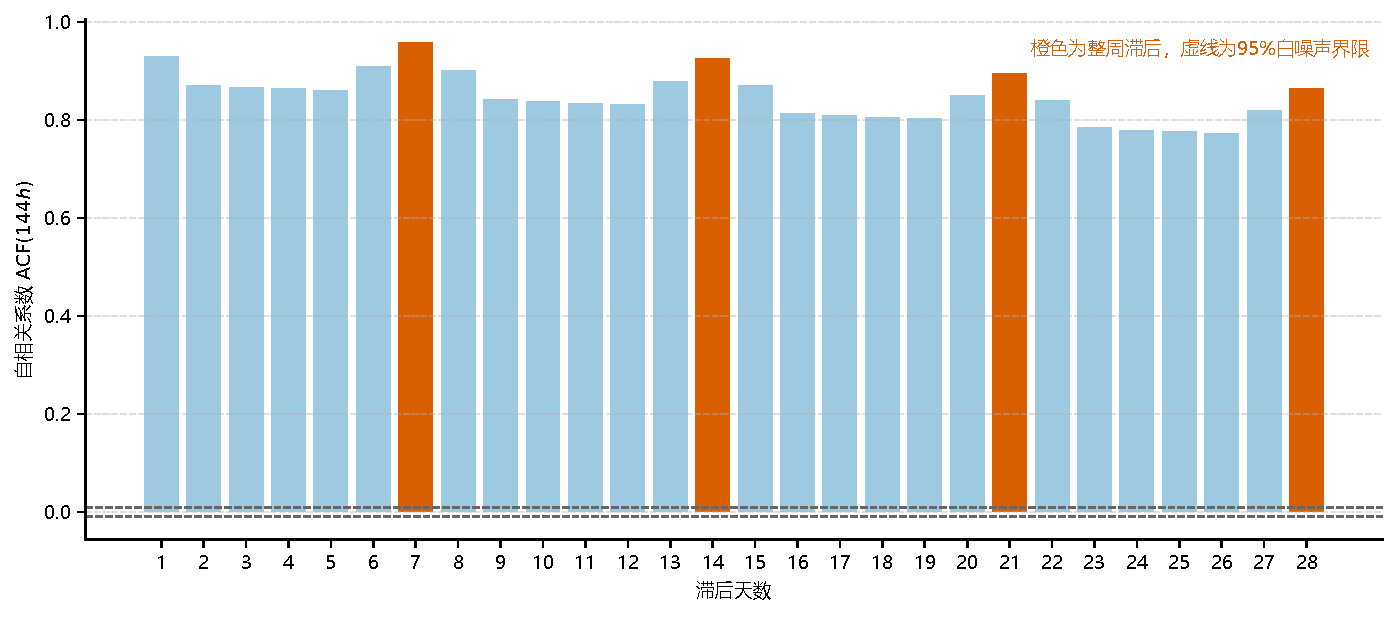
\includegraphics[width=0.485\textwidth]{../figures/问题四/问题四_ACF自相关.pdf}
  \caption{电价周期结构（左：星期一至星期日的典型电价曲线；右：整日滞后自相关函数）}
  \label{fig:q4_periodic}
\end{figure}

\subsection{0:00 固定指数周期电价预测模型}

对计划日 $d$ 的时段 $t$，使用最近至多 4 个同星期、同时刻的价格，即 $\lambda_{d-7k,t}$（$k=1,\dots,K_d$）。可用历史周数为 $K_d=\min\{4,\lfloor (d-1)/7\rfloor\}$，固定指数权重为

\begin{equation}
  w_{d,k} = \frac{\rho^{\,k-1}}{\sum_{j=1}^{K_d}\rho^{\,j-1}}, \qquad \rho = 0.8,
  \label{eq:q4_weight}
\end{equation}

式中：$w_{d,k}$ 为前第 $k$ 个同星期价格的权重；$\rho$ 为衰减系数，取 0.8，使越近的周权重越大。0:00 的电价预测为

\begin{equation}
  \widehat\lambda_{d,t}^{(0)} = \max\left\{\sum_{k=1}^{K_d} w_{d,k}\,\lambda_{d-7k,t},\ 0\right\},
  \label{eq:q4_pred0}
\end{equation}

式中：$\widehat\lambda_{d,t}^{(0)}$ 为计划日 $d$、时段 $t$ 的 0:00 电价预测值（元/kWh）；上标 $(0)$ 表示该预测在 0:00 生成；$\max\{\cdot,0\}$ 用于保证预测价格非负。当 4 周历史全部可用时，归一化权重为 $(w_1,w_2,w_3,w_4) = (0.3388,\ 0.2710,\ 0.2168,\ 0.1734)$。

样本外预测的平均绝对误差为 0.0467 元/kWh，均方根误差为 0.0665 元/kWh，WAPE（按式~\eqref{eq:wape} 计算）为 6.17\%，日内 Spearman 秩相关系数为 0.9526；前 20\% 高价时段识别率为 89.30\%，最高价时刻误差为 119.6 min。上一日同期、上一周同期和最近 4 周简单平均三个对照模型的平均绝对误差依次为 0.0843、0.0472、0.0489 元/kWh，对应秩相关系数为 0.9380、0.9460、0.9517。相较最优对照（上一周同期），四周指数加权模型使平均绝对误差降低 0.91\%，WAPE 由 6.22\% 降至 6.17\%，日内排序相关系数由 0.9460 提升至 0.9526，故用于后续储能调度；各模型误差对比如图~\ref{fig:q4_pred_err} 所示。

\begin{figure}[H]
  \centering
  
\includegraphics[width=0.72\textwidth]{../figures/问题四/问题四_电价预测模型误差对比.pdf}
  \caption{0:00 电价预测模型的误差对比}
  \label{fig:q4_pred_err}
\end{figure}

\subsection{日内因果门控的残差更新}

当天价格相对 0:00 周期基线的残差为 $e_{d,t} = \lambda_{d,t} - \widehat\lambda_{d,t}^{(0)}$。在 6:00、12:00、18:00 三个时点，模型可以使用截至决策时刻已经发生的价格残差。取滞后集合

\begin{equation}
  \mathcal J = \{1,2,3,6,12,18,36,72,144\},
  \label{eq:q4_lags}
\end{equation}

式中：$\mathcal J$ 中各元素为该时刻之前第若干个 10 分钟时段，分别对应 10 分钟至 1 天的时间尺度。建立残差自回归模型

\begin{equation}
  e_n = \beta_0 + \sum_{\ell\in\mathcal J}\beta_\ell\, e_{n-\ell} + \varepsilon_n,
  \label{eq:q4_ar}
\end{equation}

式中：$e_n$ 为第 $n$ 个时段的电价残差（元/kWh）；$\beta_0$ 为截距，$\beta_\ell$ 为各滞后阶的回归系数；$\varepsilon_n$ 为残差项。参数通过岭回归估计\cite{ref7}：

\begin{equation}
  \widehat{\boldsymbol\beta} = \arg\min_{\boldsymbol\beta}\left\{\sum_n \left(e_n-\beta_0-\mathbf x_n^{\mathsf T}\boldsymbol\beta\right)^2 + \alpha\|\boldsymbol\beta\|_2^2\right\},
  \label{eq:q4_ridge}
\end{equation}

式中：$\mathbf x_n$ 为由滞后残差构成的解释向量；$\alpha$ 为正则化参数，从 $\{0.1,1,10,20,50,100\}$ 中通过扩展窗口时间序列验证选取；参数只使用当前月份以前的数据拟合，月内固定，避免逐日重复估计带来的不稳定。

残差更新并非在所有月份都优于周期基线。为此在每月开始前，用最近 7 个可验证历史日比较残差模型与周期基线的 MAE，仅当残差模型更优时该月在该时点启用更新，即

\begin{equation}
  \widehat\lambda_{d,t}^{(\tau)} = \max\left\{\widehat\lambda_{d,t}^{(0)} + I_{d,\tau}\,\widehat e_{d,t}^{(\tau)},\ 0\right\}, \qquad t > \tau,
  \label{eq:q4_gated}
\end{equation}

式中：$\widehat\lambda_{d,t}^{(\tau)}$ 为时点 $\tau$ 更新后的电价预测（元/kWh）；$\widehat e_{d,t}^{(\tau)}$ 为残差模型的预测值；$I_{d,\tau}\in\{0,1\}$ 为门控变量，完全由历史验证结果决定，不依赖当天未来信息。各时点的启用天数与精度改善如表 12 所示。

\threelinetable{表 12\quad 日内门控残差更新的效果}{l r r r}{%
  \textbf{更新时点} & \textbf{启用更新天数} & \textbf{周期基线 MAE} & \textbf{门控更新 MAE（相对改善）}%
}{%
  6:00  & 215 & 0.0518 & 0.0487（5.97\%） \\
  12:00 & 245 & 0.0501 & 0.0457（8.80\%） \\
  18:00 & 93  & 0.0457 & 0.0455（0.35\%） \\
}

表中 MAE 的单位为元/kWh；其统计范围为各时点之后的剩余时域，并在全部 334 天上计算：启用更新的日期使用残差修正后的预测，未启用的日期保持 0:00 周期基线。6:00 与 12:00 的更新明显改善了剩余时域的价格预测，18:00 因剩余时域较短、可用的当天残差信息有限，边际改善很小。

\subsection{三类残差的联合场景生成}

电价预测误差与负荷、光伏预测误差存在相关性，若分别独立抽样可能生成``高负荷与低价格''等缺乏历史依据的场景。因此对每个历史日 $r$ 保存严格样本外的三类残差

\begin{equation}
  \left(e^L_r(t),\ e^P_r(t),\ e^{\lambda,\tau}_r(t)\right),
  \qquad
  e^{\lambda,\tau}_r(t) = \lambda_r(t) - \widehat\lambda^{(\tau)}_{r,t},
  \label{eq:q4_joint_res}
\end{equation}

式中：$e^{\lambda,\tau}_r(t)$ 为历史日期 $r$ 在时点 $\tau$ 的电价预测残差（元/kWh）。三类残差按同一个历史日期联合抽取，每个决策模型抽取 30 个历史日，重复抽中的日期按频数合并并赋予相应场景概率，从而在不改变经验分布的前提下降低混合整数规划的规模。价格场景为

\begin{equation}
  \lambda^{(\tau)}_{d,s}(t) = \max\left\{\widehat\lambda^{(\tau)}_{d,t} + e^{\lambda,\tau}_{r_s}(t),\ 0\right\},
  \label{eq:q4_price_scenario}
\end{equation}

式中：$\lambda^{(\tau)}_{d,s}(t)$ 为时点 $\tau$、计划日 $d$、场景 $s$、时段 $t$ 的电价场景（元/kWh）；$r_s$ 为本次抽中的历史日期。

\subsection{问题 4-2：单时点计划模型与结果}

问题 4-2 只使用 0:00 的周期电价预测，不引入当天残差更新，其模型结构与问题二一致，同样采用季节余弦终端软区间，只是把固定的日内电价 $\lambda(t)$ 替换为随场景变化的价格。目标函数为

\begin{equation}
  \min\left\{
    \sum_s \pi_s \sum_t\left[\lambda_{d,s}(t)G_d(t) + 5\lambda_{d,s}(t)H_{d,s}(t)\right]
    + \kappa_d\,(R_d + X_d)
  \right\},
  \label{eq:q4_obj2}
\end{equation}

式中：$\lambda_{d,s}(t)$ 为场景电价（元/kWh）；$\kappa_d$ 为终端偏离惩罚系数，其含义与式~\eqref{eq:kappa} 中的 $\kappa$ 相同，只是改用计划日之前已经发生的实际电价分位数逐日构造，同样取 $\kappa_d = 0.9\,Q_{0.90}(\lambda)$，从而不使用未来电价；终端偏离惩罚只用于决策，不计入实际支付费用。场景电量平衡同式~\eqref{eq:q2_balance}，储能状态递推、容量边界与充放电互斥约束同式~\eqref{eq:q2_soc} 与式~\eqref{eq:q2_mutex}，储电量跨日连续传递。问题 4-2 的全年结果如表 13 所示。

{\footnotesize
\threelinetable{表 13\quad 问题 4-2 全年结果}{l r l r}{%
  \textbf{指标} & \textbf{结果} & \textbf{指标} & \textbf{结果}%
}{%
  计划购电量/kWh & 22229426.39 & 正常购电费/元 & 14301863.64 \\
  紧急购电量/kWh & 305254.47 & 紧急购电费/元 & 1227651.14 \\
  富余电量/kWh & 3248071.91 & 实际总费用/元 & 15529514.78 \\
  充电量/kWh & 7089161.18 & 发生紧急购电天数 & 327 \\
  放电量/kWh & 5741741.73 & 平均日末储电量/kWh & 5975.44 \\
  12 月 31 日末储电量/kWh & 6532.02 & & \\
}
}

\subsection{问题 4-3：四时点滚动模型与结果}

问题 4-3 在 0:00 制定全天计划后，于 6:00、12:00、18:00 利用当天已观测价格与附件 3 的最新光伏预报滚动调整剩余时域。设 0:00 原计划购电量为 $G_d(t)$、调整后购电量为 $A_d(t)$，调整量为

\begin{equation}
  A_d(t) - G_d(t) = U_d(t) - V_d(t), \qquad U_d(t),\,V_d(t) \ge 0,
  \label{eq:q4_adjust}
\end{equation}

式中：$U_d(t)$ 与 $V_d(t)$ 分别为相对原计划的上调量与下调量（kWh）。在决策时点 $\tau$ 对剩余时域 $\mathcal T_\tau$ 求解

\begin{equation}
  \min\left\{
    \sum_s \pi_s \sum_{t\in\mathcal T_\tau}\left[1.5\lambda^{(\tau)}_{d,s}(t)U_d(t) - 0.5\lambda^{(\tau)}_{d,s}(t)V_d(t) + 5\lambda^{(\tau)}_{d,s}(t)H_{d,s}(t)\right]
    + \kappa_d\,(R_d^{(\tau)} + X_d^{(\tau)})
  \right\},
  \label{eq:q4_obj3}
\end{equation}

式中：方括号内三项依次为上调加价费、下调抵扣（负值）与紧急购电费（元），系数含义与问题三相同。每次求解至当天 24:00，但只执行到下一个更新时点：0:00 结果执行至 6:00，6:00 结果执行至 12:00，12:00 结果执行至 18:00，18:00 结果执行至 24:00。已执行时段的购电量、充放电量与储电量不得回溯修改，每次优化的初始储电量等于上一已执行时段的实际储电量。

四种策略费用依次为 15778106.07、15553894.38、15397581.11 和 15393286.54 元。正式 4-3 相对仅 0:00 策略节省 384819.53 元（2.44\%），紧急购电量减少 27.73\%；其中 6:00 与 12:00 更新贡献绝大部分收益，18:00 的边际改善很小。按净结算口径，4-3 的计划与调整结算费、紧急购电费分别为 14462432.65 元、930853.89 元；相对 4-2 节省 136228.24 元（0.88\%），表明波动电价下的日内滚动同样有效。

\subsubsection{指定日期的完整结果}

指定日期的购电、储能与紧急购电结果分别见表 14 至表 16。

{\scriptsize
\threelinetable{表 14\quad 问题四 4-2指定日期的购电结果}{l r r r r}{%
  \textbf{时间段} & \textbf{3 月 20 日} & \textbf{6 月 21 日} & \textbf{9 月 23 日} & \textbf{12 月 21 日}%
}{%
  10:00--10:10 & 0.00 & 0.00 & 0.00 & 0.00 \\
12:00--12:10 & 573.58 & 0.00 & 519.74 & 1004.00 \\
14:00--14:10 & 0.00 & 0.00 & 0.00 & 0.00 \\
16:00--16:10 & 486.58 & 234.98 & 561.13 & 863.31 \\
18:00--18:10 & 0.00 & 474.62 & 0.00 & 733.12 \\
20:00--20:10 & 245.31 & 0.00 & 1.68 & 0.00 \\
全天购电量/kWh & 69382.94 & 39149.55 & 72824.93 & 96979.31 \\
全天购电费/元 & 43039.58 & 19453.65 & 47391.27 & 73185.53 \\
}

}

{\tiny
\begin{center}
  {\fontsize{10.5pt}{12.6pt}\heiti\bfseries 表 15\quad 问题四 4-2指定日期的储能结果}\par
  \vspace{0.25em}
  \resizebox{\textwidth}{!}{%
  \begin{tabular}{l r r r r r r r r}
    \toprule
    & \multicolumn{2}{c}{\textbf{3 月 20 日}} & \multicolumn{2}{c}{\textbf{6 月 21 日}} & \multicolumn{2}{c}{\textbf{9 月 23 日}} & \multicolumn{2}{c}{\textbf{12 月 21 日}} \\
    \cmidrule(lr){2-3}\cmidrule(lr){4-5}\cmidrule(lr){6-7}\cmidrule(lr){8-9}
    \textbf{时间段} & \textbf{充电量/kWh} & \textbf{放电量/kWh} & \textbf{充电量/kWh} & \textbf{放电量/kWh} & \textbf{充电量/kWh} & \textbf{放电量/kWh} & \textbf{充电量/kWh} & \textbf{放电量/kWh} \\
    \midrule
    0:00-4:00 & 4574.89 & 0.00 & 0.00 & 1560.22 & 4693.29 & 0.00 & 3710.18 & 0.00 \\
4:00-8:00 & 637.77 & 5964.14 & 865.01 & 2168.11 & 833.33 & 5591.98 & 833.33 & 833.33 \\
8:00-12:00 & 5991.01 & 3192.46 & 6240.88 & 0.00 & 6068.93 & 3048.02 & 5833.33 & 7806.67 \\
12:00-16:00 & 5108.41 & 350.53 & 3277.86 & 0.00 & 4943.03 & 279.69 & 8178.38 & 2709.49 \\
16:00-20:00 & 0.00 & 6644.47 & 0.00 & 5956.18 & 0.00 & 6630.91 & 0.00 & 5605.82 \\
20:00-24:00 & 5957.42 & 1995.53 & 5475.29 & 3428.99 & 4966.73 & 2009.09 & 6217.40 & 3034.18 \\
0:00 储电量/kWh & \multicolumn{2}{c}{6682.60} & \multicolumn{2}{c}{5597.21} & \multicolumn{2}{c}{5826.04} & \multicolumn{2}{c}{6710.84} \\
24:00 储电量/kWh & \multicolumn{2}{c}{6561.68} & \multicolumn{2}{c}{5299.79} & \multicolumn{2}{c}{5670.05} & \multicolumn{2}{c}{6795.66} \\
    \bottomrule
  \end{tabular}%
  }
\end{center}
}

{\scriptsize
\threelinetable{表 16\quad 问题四 4-2指定日期的紧急购电结果}{l r l r l r l r}{%
  \textbf{3 月 20 日 时段} & \textbf{购电量/kWh} & \textbf{6 月 21 日 时段} & \textbf{购电量/kWh} & \textbf{9 月 23 日 时段} & \textbf{购电量/kWh} & \textbf{12 月 21 日 时段} & \textbf{购电量/kWh}%
}{%
  0:30-0:40 & 24.54 & 0:30-0:40 & 15.83 & 5:00-5:20 & 15.93 & 1:10-1:30 & 27.03 \\
1:20-1:40 & 44.22 & 1:30-1:50 & 22.00 & 5:50-6:00 & 2.67 & 1:40-2:00 & 18.05 \\
2:40-2:50 & 2.61 & 3:00-3:40 & 28.30 & 6:20-6:40 & 8.42 & 2:10-2:30 & 33.52 \\
3:10-3:40 & 70.70 & 6:10-6:20 & 5.12 & 7:00-7:10 & 6.32 & 3:10-3:30 & 77.84 \\
11:10-11:30 & 57.69 & 19:10-19:20 & 32.59 & 9:50-10:00 & 4.54 & 3:40-4:30 & 137.21 \\
12:40-13:00 & 97.74 &  &  & 10:10-10:20 & 13.11 & 5:10-5:30 & 21.52 \\
15:00-15:10 & 5.33 &  &  & 14:30-15:30 & 282.81 & 5:50-6:50 & 166.55 \\
15:20-16:30 & 346.56 &  &  & 16:00-16:20 & 45.40 & 7:00-7:10 & 0.68 \\
16:40-17:00 & 26.91 &  &  & 16:40-16:50 & 8.73 & 7:20-7:30 & 14.48 \\
17:10-17:30 & 11.28 &  &  & 18:40-18:50 & 9.53 & 8:00-8:10 & 6.34 \\
18:50-19:20 & 92.03 &  &  & 20:20-20:40 & 28.31 & 10:30-11:50 & 451.31 \\
20:10-20:30 & 17.74 &  &  & 21:00-21:10 & 43.75 & 13:00-13:20 & 34.61 \\
21:30-21:50 & 19.92 &  &  & 22:30-22:40 & 15.59 & 17:30-17:40 & 10.73 \\
23:40-0:00+1 & 53.62 &  &  &  &  & 18:50-19:10 & 6.86 \\
 &  &  &  &  &  & 19:50-20:10 & 56.60 \\
 &  &  &  &  &  & 22:00-22:10 & 4.07 \\
 &  &  &  &  &  & 23:00-23:10 & 9.65 \\
 &  &  &  &  &  & 23:50-0:00+1 & 7.19 \\
}
}

\subsubsection{指定日期的完整结果}

指定日期的购电、储能与紧急购电结果分别见表 17 至表 19。

{\scriptsize
\threelinetable{表 17\quad 问题四 4-3指定日期的购电结果}{l r r r r}{%
  \textbf{时间段} & \textbf{3 月 20 日} & \textbf{6 月 21 日} & \textbf{9 月 23 日} & \textbf{12 月 21 日}%
}{%
  10:00--10:10 & 0.00 / 0.00 & 0.00 / 0.00 & 0.00 / 0.00 & 0.00 / 0.00 \\
12:00--12:10 & 658.00 / 567.69 & 0.00 / 0.00 & 513.04 / 444.43 & 995.84 / 966.61 \\
14:00--14:10 & 64.20 / 0.00 & 0.00 / 0.00 & 0.00 / 0.00 & 0.00 / 0.00 \\
16:00--16:10 & 659.13 / 541.66 & 233.76 / 187.28 & 603.11 / 603.11 & 872.14 / 872.14 \\
18:00--18:10 & 0.00 / 0.00 & 514.48 / 514.48 & 6.40 / 6.40 & 725.44 / 725.44 \\
20:00--20:10 & 216.35 / 216.35 & 0.00 / 0.00 & 8.21 / 32.69 & 0.00 / 0.00 \\
全天购电量/kWh（计划 / 调整后） & 74034.74 / 69070.05 & 38182.76 / 37819.52 & 76301.19 / 74112.62 & 96829.39 / 96192.18 \\
全天购电费/元（计划 / 调整后） & 46301.64 / 44560.42 & 19316.49 / 19209.60 & 50120.63 / 49802.86 & 72877.93 / 72637.91 \\
}
单元格依次为 0:00 计划值与最终调整后执行值。
}

{\tiny
\begin{center}
  {\fontsize{10.5pt}{12.6pt}\heiti\bfseries 表 18\quad 问题四 4-3指定日期的储能结果}\par
  \vspace{0.25em}
  \resizebox{\textwidth}{!}{%
  \begin{tabular}{l r r r r r r r r}
    \toprule
    & \multicolumn{2}{c}{\textbf{3 月 20 日}} & \multicolumn{2}{c}{\textbf{6 月 21 日}} & \multicolumn{2}{c}{\textbf{9 月 23 日}} & \multicolumn{2}{c}{\textbf{12 月 21 日}} \\
    \cmidrule(lr){2-3}\cmidrule(lr){4-5}\cmidrule(lr){6-7}\cmidrule(lr){8-9}
    \textbf{时间段} & \textbf{充电量/kWh} & \textbf{放电量/kWh} & \textbf{充电量/kWh} & \textbf{放电量/kWh} & \textbf{充电量/kWh} & \textbf{放电量/kWh} & \textbf{充电量/kWh} & \textbf{放电量/kWh} \\
    \midrule
    0:00-4:00 & 4166.67 & 0.00 & 0.00 & 2771.92 & 4166.67 & 0.00 & 4166.67 & 0.00 \\
4:00-8:00 & 1217.06 & 6225.18 & 833.33 & 2101.23 & 1160.75 & 6061.42 & 446.32 & 871.02 \\
8:00-12:00 & 5305.69 & 2470.84 & 5913.23 & 0.00 & 5935.89 & 2430.50 & 5833.33 & 7448.16 \\
12:00-16:00 & 5815.79 & 366.84 & 4753.44 & 0.00 & 5463.76 & 783.26 & 7808.70 & 2736.31 \\
16:00-20:00 & 7.34 & 5901.89 & 6.30 & 5931.75 & 61.02 & 6139.65 & 16.87 & 5642.04 \\
20:00-24:00 & 6120.50 & 2745.68 & 6109.96 & 3459.73 & 4951.78 & 2513.93 & 6177.31 & 3014.38 \\
0:00 储电量/kWh & \multicolumn{2}{c}{6015.16} & \multicolumn{2}{c}{5864.61} & \multicolumn{2}{c}{6005.33} & \multicolumn{2}{c}{6648.31} \\
24:00 储电量/kWh & \multicolumn{2}{c}{6706.64} & \multicolumn{2}{c}{5869.65} & \multicolumn{2}{c}{5650.36} & \multicolumn{2}{c}{6750.47} \\
    \bottomrule
  \end{tabular}%
  }
\end{center}
}

{\scriptsize
\threelinetable{表 19\quad 问题四 4-3指定日期的紧急购电结果}{l r l r l r l r}{%
  \textbf{3 月 20 日 时段} & \textbf{购电量/kWh} & \textbf{6 月 21 日 时段} & \textbf{购电量/kWh} & \textbf{9 月 23 日 时段} & \textbf{购电量/kWh} & \textbf{12 月 21 日 时段} & \textbf{购电量/kWh}%
}{%
  0:30-0:40 & 26.81 & 0:30-0:40 & 2.65 & 5:10-5:20 & 17.28 & 0:10-0:30 & 3.85 \\
1:20-1:50 & 52.28 & 1:30-1:40 & 10.42 & 7:50-8:00 & 2.39 & 1:10-1:30 & 9.33 \\
2:40-3:00 & 8.22 & 2:20-2:30 & 0.22 & 21:00-21:20 & 39.99 & 1:40-1:50 & 6.75 \\
3:20-3:40 & 41.91 & 3:00-3:40 & 42.49 &  &  & 2:10-2:30 & 10.78 \\
5:10-5:20 & 4.25 & 19:10-19:20 & 10.45 &  &  & 3:10-3:30 & 67.44 \\
8:10-9:30 & 256.67 &  &  &  &  & 3:40-4:10 & 97.87 \\
9:50-10:10 & 75.55 &  &  &  &  & 4:20-4:30 & 0.23 \\
11:10-12:10 & 193.22 &  &  &  &  & 5:10-5:30 & 13.05 \\
12:40-13:40 & 263.99 &  &  &  &  & 5:50-6:40 & 64.34 \\
14:10-14:20 & 3.15 &  &  &  &  & 7:10-7:20 & 2.24 \\
16:10-16:30 & 26.18 &  &  &  &  & 8:00-8:10 & 3.15 \\
18:10-18:20 & 1.82 &  &  &  &  & 8:50-9:10 & 30.18 \\
18:50-19:20 & 94.52 &  &  &  &  & 9:40-10:10 & 56.21 \\
20:10-20:30 & 27.51 &  &  &  &  & 10:30-12:10 & 467.75 \\
21:30-21:50 & 19.17 &  &  &  &  & 12:50-13:20 & 18.50 \\
23:40-0:00+1 & 38.22 &  &  &  &  & 17:30-17:40 & 8.16 \\
 &  &  &  &  &  & 18:50-19:10 & 10.03 \\
 &  &  &  &  &  & 19:50-20:10 & 59.27 \\
 &  &  &  &  &  & 23:00-23:10 & 6.35 \\
 &  &  &  &  &  & 23:40-0:00+1 & 20.04 \\
}
}


2025 年 3 月 20 日的价格预测、滚动购电量与储电量轨迹如图~\ref{fig:q4_day} 所示。

\begin{figure}[H]
  \centering
  
\includegraphics[width=0.72\textwidth]{../figures/问题四/问题四_指定日价格预测与滚动调度.pdf}
  \caption{2025 年 3 月 20 日价格预测与滚动调度结果}
  \label{fig:q4_day}
\end{figure}

% 价格完全信息下界已移入第八章的方案对比，避免与敏感性分析重复。
\endinput
\subsection{价格完全信息下界}

为量化电价预测误差造成的经济损失，保持负荷与光伏场景的信息结构与现实策略一致，只把未来价格场景替换为当天的实际价格：

\begin{equation}
  \lambda_{d,s}(t) = \lambda^{\mathrm{act}}_d(t), \qquad F^{\mathrm{PI}}_{4\text{-}j}, \quad j\in\{2,3\},
  \label{eq:q4_PI}
\end{equation}

式中：$\lambda^{\mathrm{act}}_d(t)$ 为当天的实际电价（元/kWh）；$F^{\mathrm{PI}}_{4\text{-}j}$ 为价格完全信息下问题 $4\text{-}j$ 的最优费用（元）。价格信息损失定义为 $\Delta F^{\lambda}_{4\text{-}j} = F^{\mathrm{reality}}_{4\text{-}j} - F^{\mathrm{PI}}_{4\text{-}j}$，式中 $F^{\mathrm{reality}}_{4\text{-}j}$ 为现实策略的实际总费用。计算结果为：问题 4-2 的完全信息下界为 15386096.19 元，价格信息损失 143418.60 元，占下界的 0.93\%；问题 4-3 的完全信息下界为 15236867.28 元，价格信息损失 156419.25 元，占下界的 1.03\%。由于完全信息模型只放开未来实际价格，负荷与光伏仍保持现实的信息结构，该差额可解释为纯粹的价格预测误差造成的经济损失，其相对下界的差距在 1\% 左右，说明本文的周期电价预测已经捕获了绝大部分可用于储能套利的价格信息。反之，若把附件 4 的当天实际电价直接代入日前决策，得到的正是该完全信息解，它只能作为理论下界，不能当作可实施的策略。

需要说明的是，问题四使用附件 4 的实时波动电价，而问题二使用附件 1 的固定日内电价，两者的价格结构与结算口径不同，全年费用不可直接比较。附件 4 的全年平均电价与附件 1 一致（均为 0.7662 元/kWh），但其日内峰谷极差明显更大；即使给定完全信息，波动电价下的最优调度费用仍高于固定电价情形，说明电价波动本身会提高储能的调度难度与购电成本。
